\subsection{Software design}\label{sec:sysdesc}
\subsubsection{System definition}\label{sec:sysdef}
Table \ref{tab:sysdef} shows the desired systems characteristics.

A software based system to emulate keyboard based input to a vehicle video game. The system should function as a cheap alternative to vehicle game accessories like wheels and third-party hardware controllers. The user of the system should be able to pick the colors to track. The software should get input from an integrated or attached third-party webcam. The input should be a video stream of gestures given by the user. The system should function in many different environments and should consider that the users will have varying technical backgrounds. The system should provide input to a vehicle game in the form of emulated keyboard presses based on the gestures provided by the user. A PC that is capable of running common vehicle games will be required. 

\newcommand{\specialcell}[2][c]{%
  \begin{tabular}[#1]{@{}l@{}}#2\end{tabular}}
\begin{table}[h]
\centering
\begin{tabular}{l | l}
Conditions & \specialcell{The system should function in different types of environment,\\ operated by users with varying demands and technical expertise.}\\
\hline
Scope & \specialcell{Average users of vehicle based video games with limited resources\\ or will to acquire specialized third-party hardware.}\\
\hline
Technology & \specialcell{A PC capable of running video games.\\ Integrated or third party webcam attached.}\\
\hline
Objects & Camera, user, computer, video game.\\
\hline
Functionality & \specialcell{Provide input to a vehicle based video game based\\ on gestures made by a user in front of an attached webcam.}\\
\hline
Philosophy & \specialcell{Cheap alternative input method\\ for vehicle based video games.}
\end{tabular}
\caption{System definitions} \label{tab:sysdef}
\end{table}

\subsubsection{Design criteria}
Based on the system definition (section: \ref{sec:sysdef}), and the list of requirements (section: \ref{LOR}), it is possible to prioritize the different design criteria \parencite{Stage2001} of design idea one in relation to the project.

\begin{table}[h]
\begin{tabular}{| l | c | c | c | c | c |}
\hline
Criteria & Very important & Important & Less important & Irrelevant & Trivial\\
\hline
Usability & X & & & & \\
\hline
Secure & & & X & & \\
\hline
Effective & & X & & & \\
\hline
Correct & & X & & & \\
\hline
Reliable & & & X & & \\
\hline
Maintainability & & & & X & \\
\hline
Testable & X & & & & \\
\hline
Flexible & & & X & & \\
\hline
Understandable & X & & & & \\
\hline
Reusable & & X & & & \\
\hline
Integrate-able & & & X & &\\
\hline
\end{tabular}
\caption{Design criteria priorities}\label{tab:criteria}
\end{table}

\subsubsection*{Very important}
Usability, Testability, and understandability are very important criteria in regards to this design. Because the intended users of the system include all technical backgrounds, the usability and understandability of the product are very important criteria in order to make the product appear user friendly. The Primary purpose of this product in relation to the final problem statement is to be useable for testing, therefore the design should be very testable.

\subsubsection*{Important}
The effectiveness and reusability of the product are considered important criteria on the basis that the product should not, considerably, reduce the performance of the video game or be too slow to react to the users input.  The product should be as correct as possible on order to reduce biases in the testing. The product should be reusable so the product can be used as a basis for future development.

\subsubsection*{Less important}
The security of the product is considered less important on the basis that the product will not handle any user data beyond webcam input. Exploitation of the product is therefore not likely to affect the user. In relation to the final problem statement, the reliability is less important as the product is primarily intended to be used in testing. While the base design idea does include customizability, this aspect is less relevant in relation to the final problem statement. The flexibility and integration is therefore considered less important. 

\subsubsection*{Irrelevant}
The product is not intended to be redistributed, but to form a basis for further development. The maintainability of the design is therefore considered irrelevant.

\subsubsection{The technical platform}
\subsubsection*{Equipment}
The system should be developed to be compatible to the Microsoft Windows operating system. The PC should be powerful enough to run some commonly available vehicle games. 

\subsubsection*{Basic software}
The implementation will use the C++ programming and build upon the openFrameworks framework (XX). OpenFrameworks has libraries available to handle basic graphical user interface development as well as libraries to handle the interfacing with webcams and fetching video streams. We do not plan on saving any data to the computer, therefore a database will not be needed. Finally, the system should work on the Windows 7 and Windows 8 operating systems.

\subsubsection*{System interface}
Besides a PC the system will require a webcam. This webcam can be integrated or third-party. openFrameworks should handle the interface to the camera.

\subsubsection{Component architecture}

\begin{figure}[h]
\centering
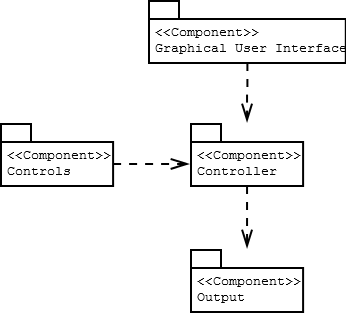
\includegraphics[scale=.8]{Components1}
\caption{System component architecture}
\label{fig:components}
\end{figure}

Figure \ref{fig:components} Shows the component architecture of the system.
The architecture will consist of several components. The graphical user interface is the component that handles communication between the user and the system, this is the component where the user will pick the colors to be tracked. The controller handles the states of the system, it is responsible for getting the tracking colors from the user, processing webcam stream, and handle the keyboard emulation. The controls component consists of classes responsible for detecting the gestures provided by the user. The output component is responsible for sending keyboard input to the video game.

\subsubsection*{Process architecture}
The system runs on a single PC with a single user. The keyboard outputs will be generated on a loop, it is therefore necessary to run this loop on a separate process in order to not lock up the main process. The webcam will be handled by the operating system and openFrameworks.

\subsubsection{User interface}
The user interface is described design one (section \ref{design1}). The interface will consist of a single window that will display the webcam image. The user will highlight the color for tracking and select the function to associate with that color.